\section*{Question 2}

\subsection*{Newton-Raphson}
Soit la fonction $G$ de la question 1. On souhaite appliquer la méthode de Newton pour trouver le point $s$ tel que $G(s)=0$. On a montrer précédemment que $G(y)=0$ ssi  $(w+ W_{\bot}y)$ est un vecteur propre de $A$. La méthode de Newton appliquée à $G$ permet donc bien de trouver le vecteur propre dominant de $A$.
Utilisons le théorème $3.10$ énoncé à la question 1.
Dans notre cas, on voit aisément que $J_G(y) = W_{\bot}^*AW_{\bot} - w^*AwI - (yw^*AW_{\bot}+Iw^*AW_{\bot}y) $ est continu en $s$ ($I$ est la matrice identité de taille $n-1$).

On peut étendre le théorème $3.10$ avec des hypothèses plus forte sur la jacobienne : 

Si, de plus, il existe une constante $\alpha > 0$ telle que la condition de Lipschitz est satisfaite
$$||DF(x) - DF(s)|| \leq \alpha || x - s||, \forall x \in \Omega,$$
alors l'ordre de convergence est au moins 2. 

Dans notre cas, en utilisant l'inégalité de Cauchy et l'inégalité triangulaire, on obtient que : 
\begin{eqnarray}
||DG(x) - DG(s)|| &=& ||W_{\perp}^{*} A W_{\perp}- w^{*} A wI - (xw^*AW_{\bot}+Iw^*AW_{\bot}x) - W_{\perp}^{*} A W_{\perp}+ w^{*} A wI + (sw^*AW_{\bot}+Iw^*AW_{\bot}s) || \\
||DG(x) - DG(s)|| &=&  ||(sw^*AW_{\bot}+Iw^*AW_{\bot}s) - (xw^*AW_{\bot}+Iw^*AW_{\bot}x) || \\
 ||DG(x) - DG(s)|| &\leq & (||w^*AW_{\bot}|| + || Iw^*AW_{\bot} ||) || x-s ||
\end{eqnarray}
Par identification on a $\alpha = ||w^*AW_{\bot}|| + || Iw^*AW_{\bot} || \geq 0$, et donc la condition de Lipschitz sur $DG(x)$ est satisfaite.On conclut qu'on a bien un ordre de convergence d'au moins 2 pour la méthode de Newton appliquée à la fonction $G$.\\

Passons à présent à l'étude numérique de la méthode. Nous séparons notre analyse en trois étapes : (1) la représentation graphique de la méthode pour une matrice $A$ de taille 3; (2) l'étude numérique de la convergence et de la vitesse de convergence de la méthode.

\subsubsection{Étude graphique}
L'interprétation graphique de la méthode de Newton appliqué à la fonction $G$ est la suivante. Contrairement à la question 1.1. où la fonction $F$ calculait un vecteur $x$ de taille $n$ (avec $A$ matrice de taille $n$) qui était le vecteur propre dominant; la fonction $G$ va fixer un vecteur $w$ de tel sorte qu'on ne doivent plus calculer qu'un vecteur $y$ (dans la base $W_{\bot}$ orthogonale à $w$) de taille $n-1$. On "perd" en quelque sorte un degré de liberté. Illustrons cela sur un cas particulier.\\

Soit $A=  \left[ 
\begin{matrix}
1 & 3 & 5 \\
-2 & 4 & 6 \\
5 & 4 & -8
\end{matrix} \right] 
, w = 
\left[ 
\begin{matrix}
1 \\
0\\
0
\end{matrix} \right] , 
W_{\bot} = 
\left[ 
\begin{matrix}
0 & 0 \\
1 & 0 \\
0 & 1 
\end{matrix} \right] , 
Q=
\left[ 
\begin{matrix}
0.2672 & 0.9094 & 0.7416 \\
0.3831 & -0.2059 & 0.5256 \\
-0.8842 & 0.3613 & 0.4169
\end{matrix} \right] 
$\\
Où $Q$ est la matrice des vecteurs propres de $A$. Les vecteurs propres sont donc des vecteurs de l'espace $\mathbb{R^3}$ (cf. figure \ref{figureNewton}). $W_{\bot}$ est un plan de normale $w$. La méthode recherche un vecteur $y$ qui appartient au plan $W_{bot}$. Ou encore $y_1$, $y2$, $y3$ sont les projections orthogonale de $v1$, $v2$ et $v3$ dans le plan $W_{\bot}$.

\begin{figure}
\centering
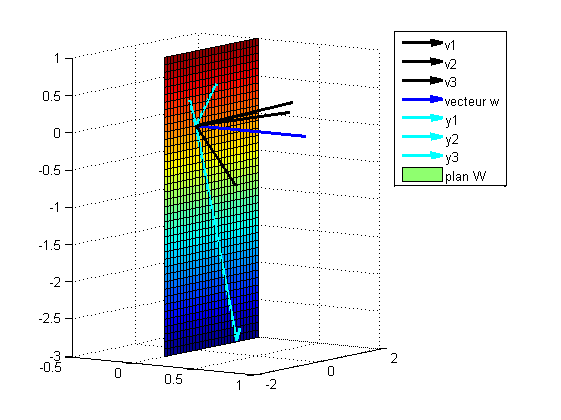
\includegraphics[width=12cm]{grapheNewton.png}\\
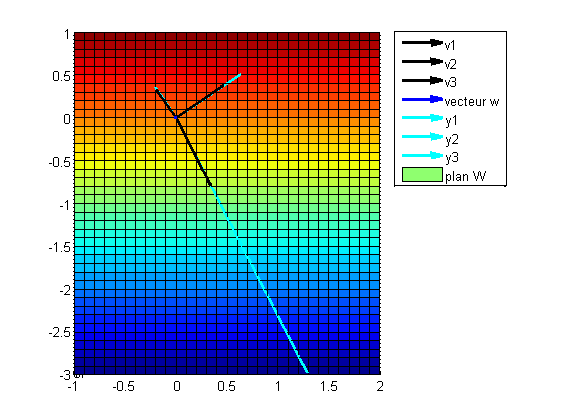
\includegraphics[width=12cm]{grapheNewton2.png}
\caption{Illustration graphique de la méthode de Newton appliquée à la fonction $G$. Le vecteur bleu est $w$ qui ets fixé. La méthode va chercher un $y_1$ (resp. $y_2$ ou $y_3$) tel que la somme vectorielle $w+y_1$ soit le vecteur propre $v_1$ (resp. $v_2$ ou $v_3$).}
\label{figureNewton}
\end{figure}

Si on représente la fonction $G$ pour ces même matrices $A$, $W_{\bot}$ et $w$, on obtient la figure \ref{grapheG}.

\begin{figure}
\centering
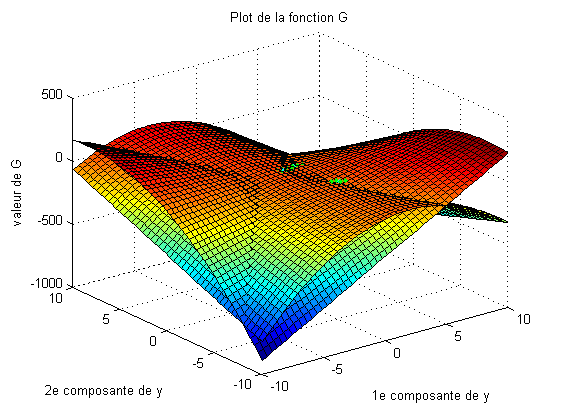
\includegraphics[width=12cm]{grapheG.png}\\
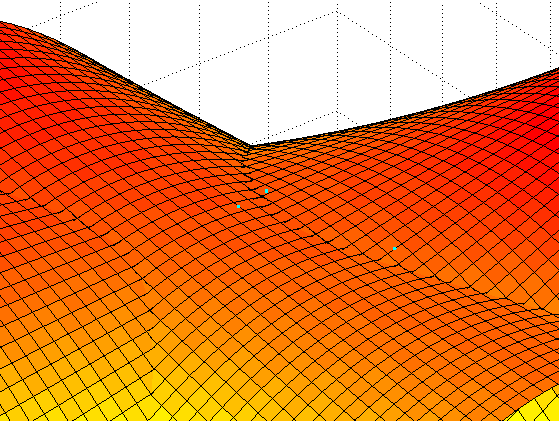
\includegraphics[width=12cm]{grapheG2.png}
\caption{Graphes de la fonction $G$. $G$ étant une fonction vectorielle à deux composante ($G(y)=[G_1(y), G_2(y)]$), nous avons tracer les deux courbes sur un même graphe. On cherche les points $y$ tels que $G_1(y)=G_2(y)=0$. Ces points sont tracer en vert sur les graphes ($G_1$ et $G_2$ étant ici tracer approximativement, ce points ne sont pas tous des racines mais permettent de localiser grossièrement les zones où se trouvent les vraies racines de $G$, ce qui est suffisant pour notre analyse), tandis que les points $y$ sont tracer en blanc.}
\label{grapheG}
\end{figure}
Graphiquement, la méthode de Newton convergera (pas toujours, selon les bassins de convergence de la méthode) vers un $y$ le plus proche de $y_0$, l'itéré de départ.\\



Regardons ce qui se passe quand $w$ est orthogonal au vecteur propre dominant. Cela signifie que $v_1$ est dans le plan $W_\bot$. Par conséquent, on ne peut exprimer $v_1$ par $w+W_{\bot}y$ (sauf peut-être pour $||y|| \rightarrow \infty$). \\
Soit $w = 
\begin{bmatrix}
1 \\
0\\
0.3021
\end{bmatrix} , 
W_{\bot} =  
\begin{bmatrix}
0 & 0.2672 \\
1 & 0 \\
0 & -0.8842 
\end{bmatrix}$\\
La fonction $G$ n'a plus que deux racines (cf. figure \ref{FigNewtonv1inW}).

\begin{figure}
\centering
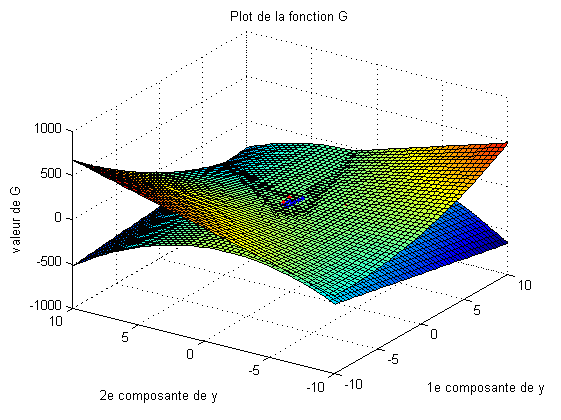
\includegraphics[width=12cm]{grapheG3.png}
\caption{Graphe de $G$ pour la même matrice $A$, mais pour $v_1 \bot w$  
}
\label{FigNewtonv1inW}
\end{figure}


\subsubsection{Étude de la convergence}
Prenons une matrice aléatoire $A$ de taille 5 (randn(5)). Soit $w=[1,0,0,0,0]$ et $W_{\bot}$ sont complément orthogonal. Appliquons la méthode de Newton. Si celle-ci converge nous obtenons une erreur du type : 
\begin{table}
\centering
\begin{tabular}{cccc}
itération & erreur (sur $y+$) & itération & erreur\\
\end{tabular}
\end{table}  

\paragraph{Remarque : }
Observons un phénomène numérique intéressant : si on impose une trop grande précision à la méthode de Newton (ex : $\epsilon = 1e-30$), on a une stagnation de l'erreur qui apparaît (cf. figure \ref{plor_erreur}). Cela est du au fait que notre itération de Newton est définie comme : $x_{k+1} = x_k - J_G^{-1}(xk) G(x_k)$. le fait qu'on fasse une différence implique une perte de précision à partir d'un certain nombre d'itération. D'où l'intérêt des méthodes d'extrapolation (type Aiteken ou Steffesen). 

\begin{figure}
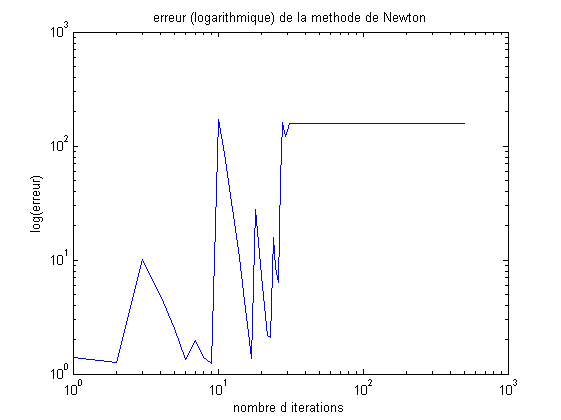
\includegraphics[width = 12cm]{erreur.png}
\caption{Plot logarithmique de l'erreur à chaque itération.}
\label{plor_erreur}
\end{figure}

\subsection*{Rayleigh symétrique}
On peut voir la méthode de Rayleigh comme une méthode de la puissance avec un "shift" variable (mis a jour à chaque itération). En d'autre mots, elle définie la méthode itérative suivante : 
$$x_{k+1} = \left(  A- \frac{x^*Ax}{x^*x}  \right)^{-1} x_k.  $$
\textbf{Proposition 4.4} Soit $A = A^*$ $ \in \mathbb{C}^{n\times n}$. L'itération du quotient de Rayleigh pour $A$ converge vers une direction propre de $A$ pour presque tout itéré initial. Lorsque la suite des itérés converge vers une direction propre, la convergence est cubique. 

Il faut maintenant préciser ce \textit{pour presque tout itéré initial}. Supposons que $A$ est diagonalisable et faisons un changement de variable afin d'exprimer $x$ dans la base formée par les vecteurs propres de $A$. Nommons le $x$ après changement de variables $x'$. Soit $Q$ la matrice dont les colonnes sont les vecteurs propres de $A$ et $D$ la matrice diagonale des valeurs propres de $A$. On utilise le théorème spectrale et le fait que $A$ et $(A-\mu I)^{-1}$ possèdent les mêmes vecteurs propres pour réécrire l'itération : 
\begin{eqnarray}
Qx_{k+1}' & = &(Q D Q^T - \frac{x_k'^* D x_k}{x_k'^* x_k})^{-1} Qx_{k}'\\
Qx_{k+1}' & = & Q(D-\frac{x_k'^* D x_k}{x_k'^* x_k})^{-1}Q^T Qx_k'\\
x_{k+1}' & = & \underbrace{(D-\frac{x_k'^* D x_k}{x_k'^* x_k})^{-1}}_{\text{matrice diagonale}} x_k'
\end{eqnarray}
Supposons qu'on souhaite converger vers le vecteur propres dominant $v_1$, autrement dit on souhaite que $lim_{k\rightarrow \infty} x_k' = [1 0 \cdots 0]^T$. Pour que cela soit possible, il faut que $x_0$ ait sa composante dans la direction $v_1$ non nulle ($x_0'^* v_1 \neq 0$). 

Vérifions maintenant de manière numérique les résultats théoriques obtenus. Prenons par exemple la matrice symétrique $A$ : 

$$ A = \left[
\begin{array}{ccc}
  2 & 4 & 6  \\
  4 & 2 & 1 \\
  6 & 1 & 2 \\
\end{array}
\right]$$

En utilisant la fonction $eigs$ de \textit{Matlab}, on sait que les valeurs propres de $A$ sont : 
   \begin{eqnarray*}
   \lambda_1 &=& 9.6965\\
   \lambda_2 &=& 1.0796 \\
   \lambda_3 &=& -4.7762
   \end{eqnarray*}

En appliquant l'itération du quotient de Rayleigh symétrique implémentée par nos soins pour un $x_0$ tel que : 
$$ x_0 = \left[
\begin{array}{c}
  \frac{1}{\sqrt{3}}  \\
  \frac{1}{\sqrt{3}} \\
  \frac{1}{\sqrt{3}} \\
\end{array}
\right]$$
 et pour $\mu_0 = 1000$ (la valeur propre la plus "proche" est donc 9.696530) , on obtient : 
$$\begin{array}{ccc}
  itération & erreur & \mu  \\
  1 &  990.658295   & \underline{9}.341705  \\
  2 &   0.354404   &  \underline{9.696}109\\
  3 &  0.000421  & \underline{9.696530} \\
  4 &  0.000000  & \underline{9.696530} \\
\end{array}$$

Ce qui correspond bien à la théorie. En effet, à chaque itération on gagne bien 3 chiffres significatifs comme l'illustrent l'erreur (définie comme la différence entre les $\mu_k$ à chaque itération) et les chiffres soulignés qui représentent les chiffres significatifs du $\mu_k$.

On considère maintenant un itéré initial qui n'a pas de composante dans la direction du vecteur propre  

$$ v_1 = \left[
\begin{array}{c}
  0.6834  \\
   0.4317 \\
   0.5888 \\
\end{array}
\right], \text{ t.q. } Av_1 = \lambda_1 v_1,$$

par exemple  :

$$ x_0 = \left[
\begin{array}{c}
  1  \\
  0 \\
  -1.1606\\
\end{array}
\right]$$

Lorsqu'on applique l'itération, on ne converge effectivement plus vers $\lambda_1$ mais vers $\lambda_3$. Le \textit{pour presque tout itéré initial} est donc confirmé.

\textbf{je sais ces image et explications puent pour l'instant, je les mets parce que j'ai fait le script et tout mais en soit hesitez pas à modifier et vu qu'elles vont peut etre disparaitre du rapport ca me soule d'écrire un roman pour l'expliquer nickel :p}

L'image suivante illustre les valeurs propres (sur l'axe des z, 9.6965 1.0796 -4.7762 ) vers lesquelles on converge pour différents vecteurs propres initiaux $x_0$ (représentés par les points 1, 2 ou 3 sur l'axe des x, cf. code pour savoir leur valeurs exactes) et pour différents $\mu$ initiaux (de -10 à 10 sur l'axe des y).

\begin{figure}
  \centering
  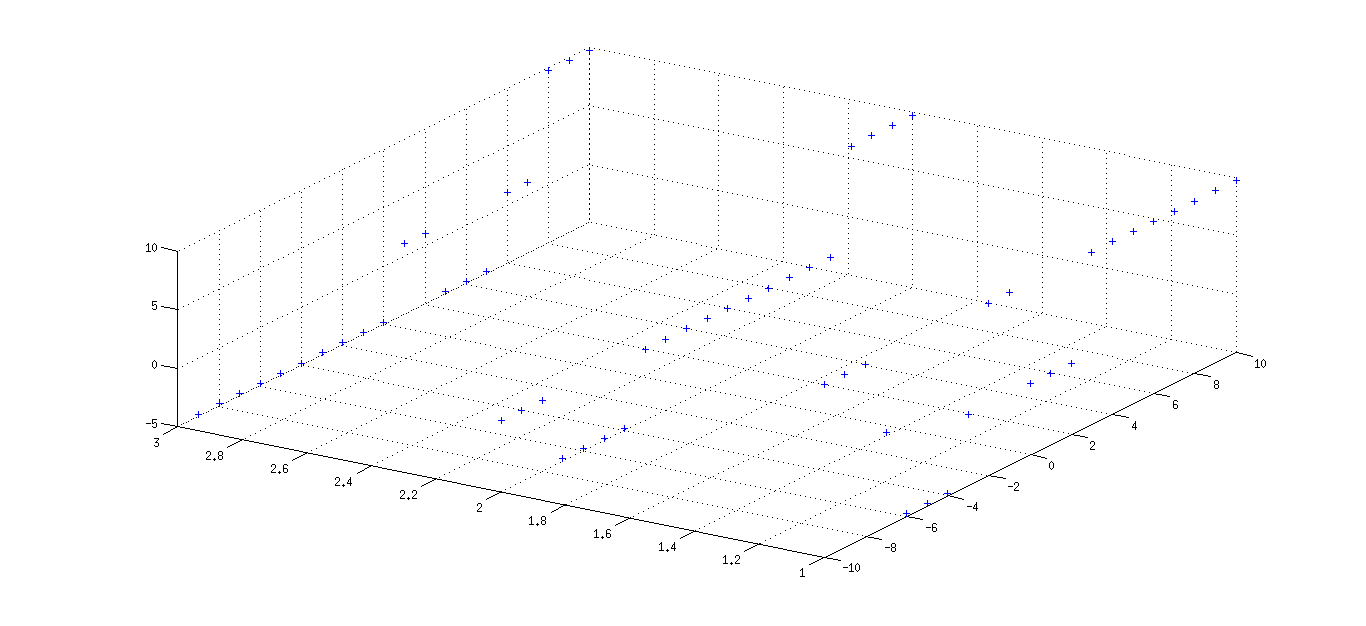
\includegraphics[width=15cm]{RaySym.png}
  \caption{Graphe représentant les valeurs propres vers lesquelles on converge pour différents $x_0$ et $mu$}
  \label{fig:RaySym}
\end{figure}
\subsection*{Rayleigh asymétrique}

